%%%%%%%%%%%%%%%%%%%%%%%%%%%%%%%%%%%%%%%%%%%%%%%%%%%%%%%%%%%%%%%%%%%%%%%%%%%%%%%%%%%%%%%%%%
% Based template: https://www.overleaf.com/latex/templates/uct-report-template/grctkzjtrqrm
%%%%%%%%%%%%%%%%%%%%%%%%%%%%%%%%%%%%%%%%%%%%%%%%%%%%%%%%%%%%%%%%%%%%%%%%%%%%%%%%%%%%%%%%%%
\documentclass[12pt]{article}
\usepackage[spanish]{babel}
\usepackage{natbib}
\usepackage{url}
\usepackage[utf8x]{inputenc}
\usepackage{amsmath}
\usepackage{graphicx}
\usepackage{float}
\usepackage{parskip}
\usepackage{fancyhdr}
\usepackage{vmargin}
\setmarginsrb{3 cm}{2.5 cm}{3 cm}{2.5 cm}{1 cm}{1.5 cm}{1 cm}{1.5 cm}

\title{DFPGA - ''Discrete FPGA''} % Title
\author{Aguilar Enriquez, Paul Sebastian \\ Cabrera Lopez, Oscar Emilio}  % Author
\date{\today} % Date

\makeatletter
\let\thetitle\@title
\let\theauthor\@author
\let\thedate\@date
\makeatother

\pagestyle{fancy}
\fancyhf{}
\rhead{\theauthor}
\lhead{\thetitle}
\cfoot{\thepage}

\begin{document}

%%%%%%%%%%%%%%%%%%%%%%%%%%%%%%%%%%%%%%%%%%%%%%%%%%%%%%%%%%%%%%%%%%%%%%%%%%%%%%%%%%%%%%%%%
\begin{titlepage}
    \centering
    
    \par
    \raisebox{-.5\height}{
\includegraphics[width=4cm]{escudo-unam.png}} % University Logo
    \hfill
    \raisebox{-.5\height}{
\includegraphics[width=4cm]{escudo-unam.png}} % Faculty Logo
    \par
    
    \hfill \break
    
    \textsc{\LARGE Universidad Nacional Autónoma de México}\\[2.0 cm]   % University Name
    \textsc{\Large Facultad de Ingeniería}\\[0.5 cm]                    % Course Code
    \textsc{\large Diseño de Sistemas Digitales}\\[0.5 cm]              % Course Name
    \rule{\linewidth}{0.2 mm} \\[0.4 cm]
    { \huge \bfseries \thetitle}\\
    \rule{\linewidth}{0.2 mm} \\[1.5 cm]
    
    \begin{minipage}{0.4\textwidth}
        \begin{flushleft} \large
            \emph{Integrantes:}\\
            \theauthor
        \end{flushleft}
    \end{minipage}~
    \begin{minipage}{0.4\textwidth}
        \begin{flushright} \large
            \emph{Codigo de Cuenta:} \\
            415028130\\312333261                                   % Your Student Number
        \end{flushright}
    \end{minipage}\\[2 cm]
    
    \begin{minipage}{0.4\textwidth}
        \begin{flushleft} \large
            \emph{Profesor:}\\
            M.I. Vicente Flores Olvera
        \end{flushleft}
    \end{minipage}~
    \begin{minipage}{0.4\textwidth}
        \begin{flushright} \large
            \emph{Fecha de entrega:}\\
            {\large \thedate}\\[2 cm]
        \end{flushright}
    \end{minipage}\\[2 cm]
    
    
    %{\large \thedate}\\[2 cm]
 
    \vfill
    
\end{titlepage}

%%%%%%%%%%%%%%%%%%%%%%%%%%%%%%%%%%%%%%%%%%%%%%%%%%%%%%%%%%%%%%%%%%%%%%%%%%%%%%%%%%%%%%%%%

\tableofcontents
\pagebreak

%%%%%%%%%%%%%%%%%%%%%%%%%%%%%%%%%%%%%%%%%%%%%%%%%%%%%%%%%%%%%%%%%%%%%%%%%%%%%%%%%%%%%%%%%

\section{Descripción del problema}

Implementar un FPGA con lógica  discreta utilizando completamente circuitos integrados de la familia 74XXX.

\section{Teoría}

\subsection{Definición de FPGA}
Los FPGA (Field Programmable Gate Arrays) son dispositivos prefabricados que pueden ser programados eléctricamente en al momento para convertirse en casi cualquier tipo de circuito o sistema digital. Para producciones de volumen bajo a medio, los FPGAs ofrecen soluciones más baratas y un tiempo de comercialización más rápido en comparación con los Circuitos Integrados de Aplicación Específica (ASIC), que normalmente requieren una gran cantidad de recursos en términos de tiempo y dinero para obtener el primer dispositivo. Los FPGAs por otro lado toman menos de un minuto para configurar y suelen tener un costo economico menor. También para diversos requisitos, una parte del FPGA se puede reconfigurar parcialmente mientras que el resto del FPGA sigue funcionando. Cualquier actualización futura en el producto final se puede actualizar fácilmente simplemente descargando un nuevo flujo de bits que representan la aplicación. La principal ventaja de los FPGAs es la flexibilidad.

La naturaleza flexible de los FPGAs los hace significativamente más grandes, más lentos y consumen más energía que sus equivalentes ASIC. Los FPGAs presentan una alternativa convincente para la implementación de sistemas digitales debido a su menor tiempo de comercialización y bajo costo de volumen.

Normalmente los FPGAs se comprenden de:
 \begin{itemize}
   \item Bloques lógicos programables que implementan funciones lógicas.
   \item Enrutamiento programable que conecta estas funciones lógicas.
   \item Bloques de E/S que están conectados a bloques lógicos a través de la interconexión de enrutamiento y que hacen conexiones tipo off-chip.
 \end{itemize}

Un ejemplo generalizado de un FPGA se muestra en la Fig. \ref{fig:1} donde los bloques lógicos configurables (CLBs) están dispuestos en una rejilla bidimensional y están interconectados por recursos de enrutamiento programables. Los bloques de E/S están dispuestos en la periferia de la rejilla y también están conectados a la interconexión de enrutamiento programable. El término ''programable/reconfigurable'' en FPGAs indica su capacidad para implementar una nueva función en el chip después de su fabricación. La reconfigurabilidad/programación de un FPGA se basa en una tecnología de programación subyacente, que puede causar un cambio en el comportamiento de un chip pre-fabricado después de su fabricación.


\begin{figure}[H]
  \centering
  %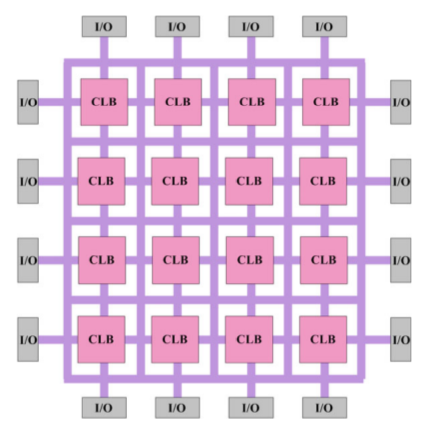
\includegraphics[height=5.5cm]{1-Overview-of-FPGA-architecture.png}
  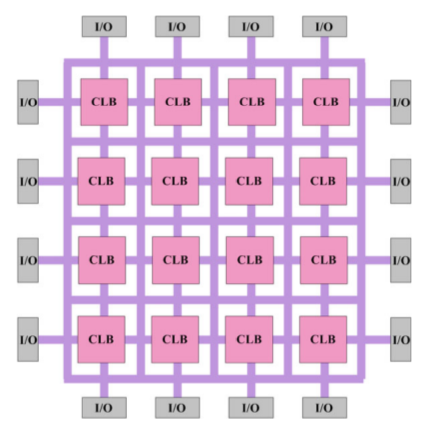
\includegraphics[]{1-Overview-of-FPGA-architecture.png}
  \caption{Vista de la arquitectura básica de un FPGA.}
  \label{fig:1}
\end{figure}

\subsection{Bloque lógico configurable}

Un bloque lógico configurable (CLB) es un componente básico de un FPGA que proporciona la lógica básica y la funcionalidad de almacenamiento para el diseño de la aplicación objetivo. Con el fin de proporcionar la lógica básica y la capacidad de almacenamiento, el componente básico puede ser un transistor o un procesador entero. Sin embargo, estos son los dos extremos donde en un extremo el componente básico es de grano fino (en el caso de transistores) y requiere una gran cantidad de interconexión programable que finalmente resulta en un FPGA que sufre ineficiencia de área, bajo rendimiento y alta potencia consumo. En el otro extremo (en el caso del procesador), el bloque lógico básico es muy grueso y no se puede usar para implementar pequeñas funciones ya que conducirá a desperdicio de recursos.

Entre estos dos extremos, existe un espectro de bloques lógicos básicos. Algunos de ellos incluyen bloques lógicos que están hechos de puertas NAND, una interconexión de multiplexores, tabla de consulta (Lookup Table - LUT) y puertas de entrada ancha de estilo PAL. Los vendedores comerciales como Xilinx y Altera utilizan CLBs basados ​​en LUT para proporcionar lógica básica y funcionalidad de almacenamiento. Los CLBs basados ​​en LUT proporcionan un buen equilibrio entre los bloques lógicos de grano demasiado fino y demasiado grueso. Un CLB puede comprender un único elemento lógico básico (Basic Logic Element - BLE), o un grupo de BLEs interconectadas localmente (como se muestra en la figura \ref{fig:2}). Un BLE simple consiste en un LUT, y un flip-flop. Un LUT con \textit{k} entradas (LUT-k) contiene $2^{k}$ bits de configuración y puede implementar cualquier función booleana de k-entradas. La Figura \ref{fig:3} muestra un BLE simple que comprende un LUT de 4 entradas (LUT-4) y un Flip-Flop de tipo D. El LUT-4 utiliza 16 bits SRAM para implementar cualquier función booleana de 4 entradas. La salida de LUT-4 está conectada a un Flip-Flop opcional. Un multiplexor selecciona la salida BLE para ser la salida de un flip-flop o el LUT-4.

\begin{figure}[H]
  \centering
  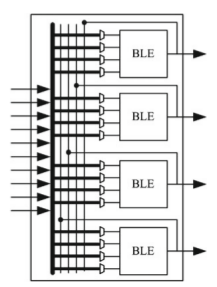
\includegraphics[]{2-CLB-having-four.png}
  \caption{Bloque lógico configurable (CLB) con cuatro BLEs}
  \label{fig:2}
\end{figure}

\begin{figure}[H]
  \centering
  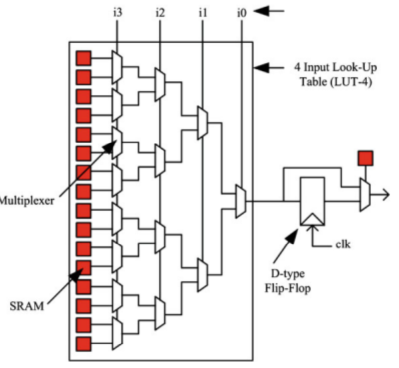
\includegraphics[height=8cm]{3-Basic-logic-element.png}
  \caption{Bloque lógico configurable (CLB) básico}
  \label{fig:3}
\end{figure}

\subsection{Arquitecturas de enrutamiento FPGA}

En un FPGA, la funcionalidad de cálculo es proporcionada por sus bloques lógicos programables y estos bloques se conectan entre sí a través de la red de enrutamiento programable. Esta red de encaminamiento programable proporciona conexiones de enrutamiento entre bloques lógicos y bloques de E/S para implementar cualquier circuito definido por el usuario.

La interconexión de enrutamiento de un FPGA consiste en cables y interruptores programables que forman la conexión requerida. Estos interruptores programables se configuran utilizando la tecnología programable.


Dado que las arquitecturas FPGA afirman ser un candidato potencial para la implementación de cualquier circuito digital, su interconexión de enrutamiento debe ser muy flexible para que puedan acomodar una amplia variedad de circuitos con demandas de enrutamiento muy variadas. Aunque los requerimientos de enrutamiento varían de circuito a circuito, ciertas características comunes de estos circuitos pueden usarse para diseñar óptimamente la interconexión de enrutamiento de la arquitectura FPGA.

Por ejemplo, la mayoría de los diseños muestran localidad, por lo que requieren abundantes cables cortos. Pero al mismo tiempo hay algunas conexiones distantes, lo que lleva a la necesidad de cables largos y escasos. Por lo tanto, el cuidado debe tenerse en cuenta al diseñar la interconexión de enrutamiento para las arquitecturas FPGA donde tenemos que abordar la flexibilidad y la eficiencia. La disposición de recursos de encaminamiento, relativa a la disposición de bloques lógicos de la arquitectura, juega un papel muy importante en la eficiencia global de la arquitectura. Esta disposición se denomina aquí como arquitectura de enrutamiento global, mientras que los detalles microscópicos relativos a la topología de conmutación de diferentes bloques de conmutación se denominan arquitectura de enrutamiento detallada. Sobre la base de la disposición global de los recursos de enrutamiento de la arquitectura, las arquitecturas FPGA pueden clasificarse como de tipo jerárquico o de isla, no se abundara en los calsificaciones.

\begin{figure}[H]
  \centering
  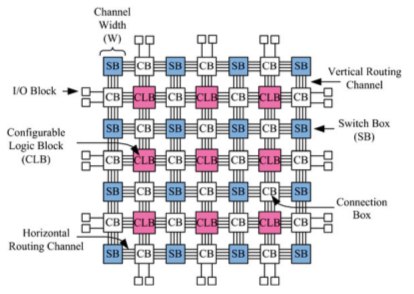
\includegraphics[]{4-Overview-of-mesh-based-FPGA-architecture.png}
  \caption{Vista de la arquitectura de un FPGA basado en malla.}
  \label{fig:4}
\end{figure}

\subsection{Arquitectura Asíncrona FPGA}

Otro enfoque alternativo que se ha propuesto para mejorar el rendimiento general de la arquitectura FPGA es el uso de elementos de diseño asíncrono.

Convencionalmente, los circuitos digitales están diseñados para la operación síncrona ya su vez las arquitecturas FPGA se han centrado principalmente en la implementación de circuitos síncronos. Se proponen diseños asíncronos para mejorar la eficiencia energética de los FPGA asincrónicos, ya que los diseños asíncronos ofrecen energía potencialmente menor, ya que la energía se consume sólo cuando sea necesario. También las arquitecturas asíncronas pueden simplificar el proceso de diseño ya que las complejas redes de distribución de reloj se vuelven innecesarias.

\subsection{Programación}

En el FPGA no se realiza programación tal cual como se realiza en otros dispositivos como DSP, CPLD o microcontroladores. El FPGA tiene celdas que se configuran con una función específica ya sea como memoria (FLIP-FLOP tipo D), como multiplexor o con una función lógica tipo AND, OR, XOR. La labor del ''programador'' es describir el hardware que tendrá la FPGA. 

El diseñador cuenta con la ayuda de entornos de desarrollo especializados en el diseño de sistemas a implementarse en un FPGA. Un diseño puede ser capturado ya sea como esquemático, o haciendo uso de un lenguaje de programación especial. Estos lenguajes de programación especiales son conocidos como HDL o Hardware Description Language (lenguajes de descripción de hardware). Los HDLs más utilizados son:

\begin{itemize}
  \item VHDL
  \item Verilog
  \item ABEL
\end{itemize}

En un intento de reducir la complejidad y el tiempo de desarrollo en fases de prototipaje rápido, y para validar un diseño en HDL, existen varias propuestas y niveles de abstracción del diseño. Los niveles de abstracción superior son los funcionales y los niveles de abstracción inferior son los de diseño al nivel de componentes hardware básicos.

\section{Método de solución}



\section{Código}



\section{Construcción Virtual}



\section{Conclusión}



\bibliographystyle{plain}
\bibliography{biblist}

\end{document}
